\section*{Результат работы программы.}
\begin{enumerate}
	\item Графики зависимости от времени импульса $t$: $I(t), U(t), R_p(t),$ произведения $I(t) \cdot R_p(t), T_0(t)$ при заданных выше параметрах.
	Шаг сетки - $10^{-7}$.
	
	\begin{figure}[h]
		\begin{center}
			{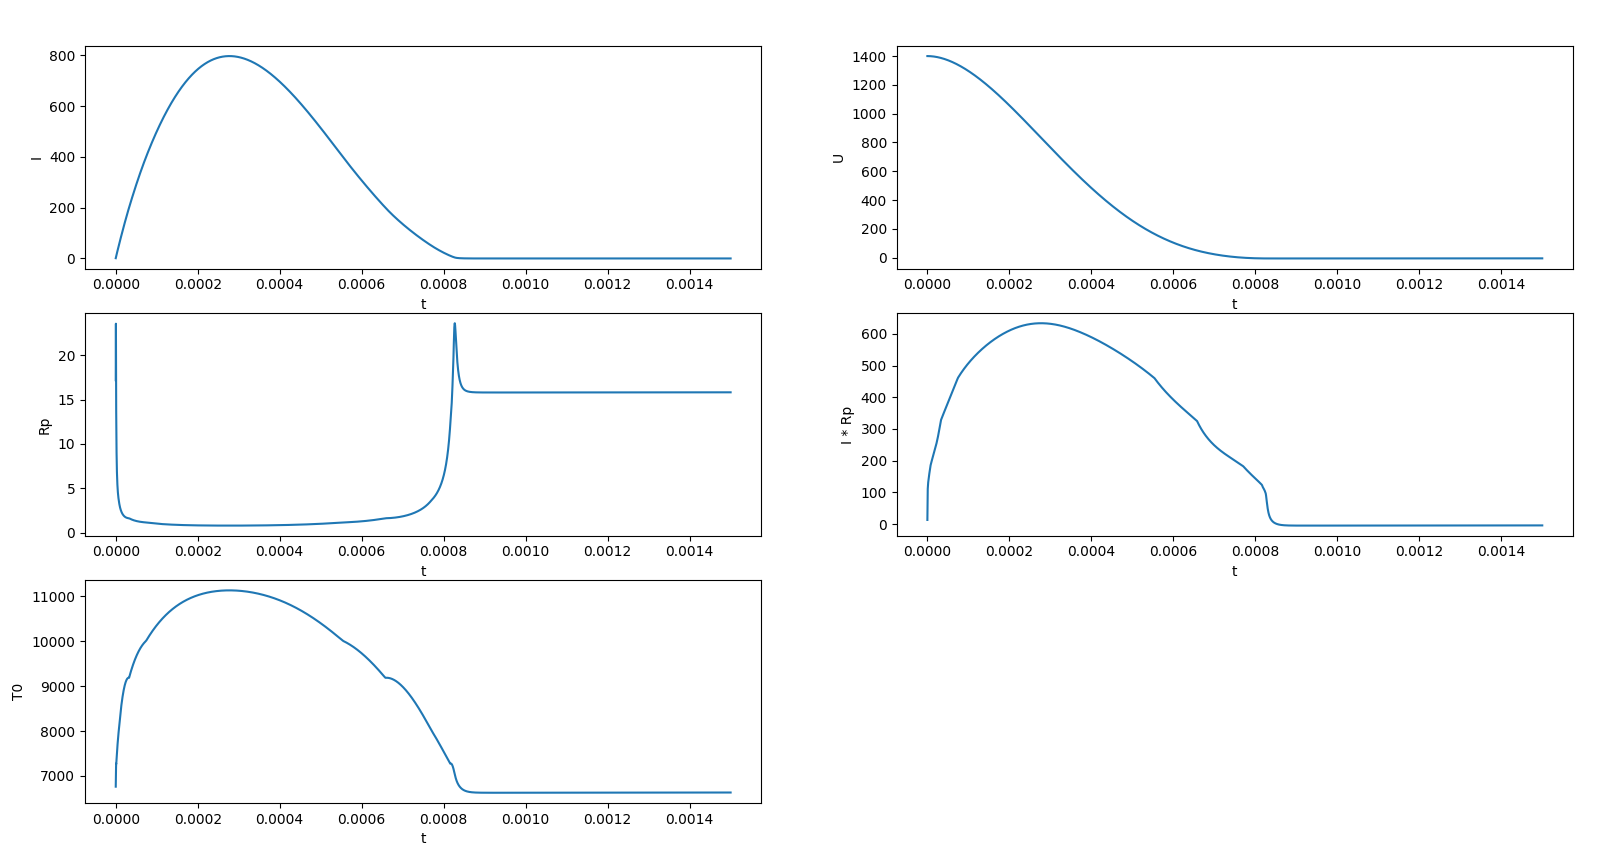
\includegraphics[height=9.5cm, width = 18cm]{tasks/task_1}}
		\end{center}
	\end{figure}
	
	\item График зависимости $I(t)$ при $R_k + R_p = 0$. Обратить внимание на то, что в этом случае колебания тока будут незатухающими.
	
	\begin{figure}[h]
		\begin{center}
			{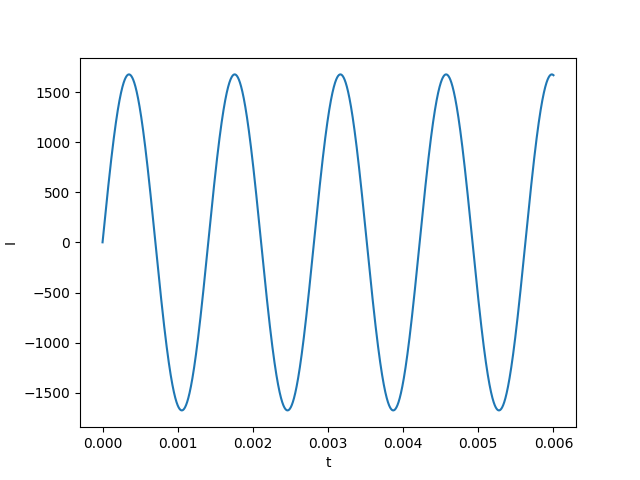
\includegraphics[height=9cm, width = 16cm]{tasks/task_2}}
		\end{center}
	\end{figure}
	
	\item График зависимости $I(t)$ при $R_k + R_p = const = 200$ Ом в интервале значений $t$ 0-20 мкс.
	
	\begin{figure}[h]
		\begin{center}
			{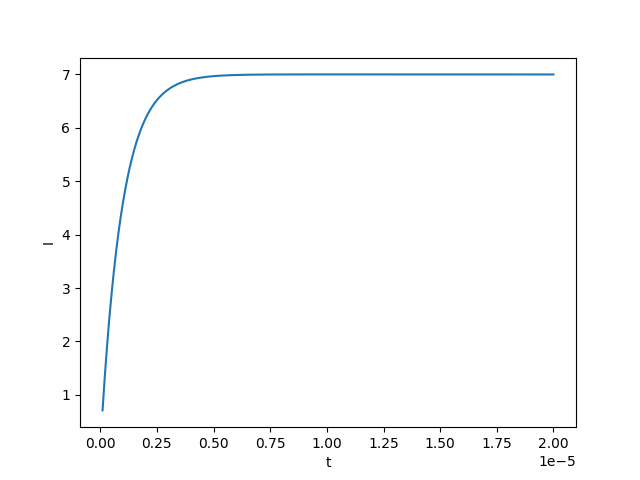
\includegraphics[height=7.76cm, width = 16cm]{tasks/task_3}}
		\end{center}
	\end{figure}
	
	\item Результаты исследования влияния параметров контура $C_k, L_k, R_k$ на длительность импульса tимп. апериодической формы. Длительность импульса определяется по кривой зависимости тока от времени на высоте
	$35 I_{max}, I_{max}$ - значение тока в максимуме (см. рисунок).
	
	\begin{figure}[h]
		\begin{center}
			{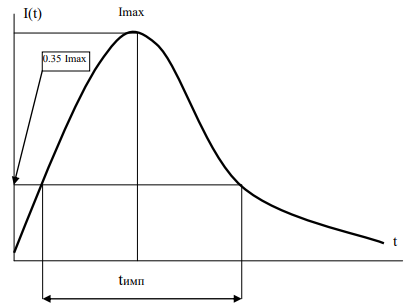
\includegraphics[height=3.3cm, width =8cm]{graph}}
		\end{center}
	\end{figure}
	
	\begin{table}[ph!]\label{table_3}
		\caption{Влияние $C_k$ на длительность импульса tимп}
		\centering
		\begin{tabular}{|c|c|c|c|c|c|c|c|c|c|c|}
			\hline
			$C_k$, мкФ & 200 & 250 & 300 & 350 & 400 & 450 & 500 & 550 & 600 & 650\\
			\hline
			tимп, мкс & 485.10 & 546.10 & 602.10 & 654.20 & 703.20 & 749.90 & 794.70 & 838.0 & 879.70 & 920.40\\
			\hline	
		\end{tabular}
	\end{table}
	
	\begin{table}[ph!]\label{table_4}
		\caption{Влияние $L_k$ на длительность импульса tимп}
		\centering
		\begin{tabular}{|c|c|c|c|c|c|c|c|c|c|c|}
			\hline
			$L_k$, мкГн & 100 & 150 & 200 & 250 & 300 & 350 & 400 & 450 & 500 & 550 \\
			\hline
			tимп, мкс & 425.50 & 511.80 & 584.70 & 649.30 & 708.20 & 762.50 & 813.20 & 861.00 & 906.20 & 949.20\\
			\hline	
		\end{tabular}
	\end{table}
	
	\begin{table}[ph!]\label{table_5}
		\caption{Влияние $R_k$ на длительность импульса tимп}
		\centering
		\begin{tabular}{|c|c|c|c|c|c|c|c|c|c|c|c|}
			\hline
			$R_k$, Ом & 0.1 & 0.2 & 0.4 & 0.6 & 0.8 & 1.0 & 1.2 & 1.4 & 1.6 & 1.8 & 2.0 \\
			\hline
			tимп, мкс & 556.20 & 562.90 & 580.2 & 604.5 & 636.3 & 675.3 & 723.9 & 781.01 & 842.6 & 903.2 & 959.7\\
			\hline	
		\end{tabular}
	\end{table}
	
	\begin{figure}[ph!]
		\begin{center}
			{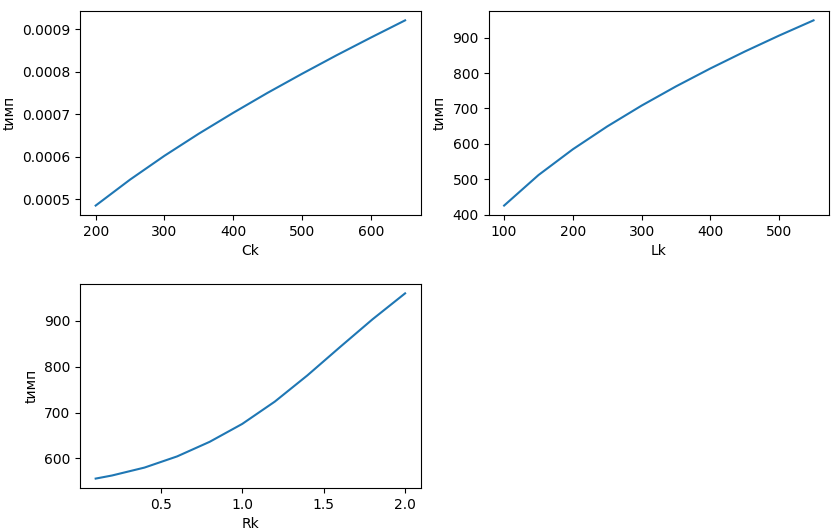
\includegraphics[height=7.58cm, width = 16cm]{tasks/task_4}}
		\end{center}
	\end{figure}
	В результате исследования было выявлено, что при увеличении любого из трёх параметров увеличивается и длительность импульса.
	
\end{enumerate}